设计、实现和维护软件项目的难度与复杂性有关。我们可以使用面向过程的方法(即过程编程范式)编写一个简单的计算器,但用相同的方法实现银行账户管理系统就会非常复杂。 \par
C++支持面向对象编程(OOP),这种范式建立在将实体分解为对象的基础上。想象一下在现实世界中一个简单的场景,当你拿着遥控器换电视频道时。至少有三种不同的物体参与这个动作:遥控器、电视,还有你自己。为了使用编程语言表达现实世界的对象关系,我们不必使用类、继承、抽象、接口、虚函数等等。上面提到的特性和概念将程序设计为过程式会更容易,因为它们允许我们以优雅的方式表达想法,但并不强制。正如C++的创始人Bjarne Stroustrup所说:“并不是每个程序都应该面向对象。”为了理解OOP范式的高级概念和特性,我们将尝试从了解其背后的信息。本书中,我们将深入研究面向对象程序的设计。理解对象关系的本质,然后使用它们来设计面向对象的程序。 \par
本章中,我们将了解以下内容: \par

\begin{itemize}
	\item 了解面向对象编程
	\item C++对象模型
	\item 类关系,包括继承
	\item 多态性
	\item 有用的设计模式
\end{itemize}

\noindent\textbf{}\ \par
\textbf{编译器要求} \ \par
g++编译器需要添加编译选项 \texttt{-std=c++2a} 来编译本章的代码。可以从这里获取本章的源码文件:https:/​/github.​com/PacktPublishing/Expert-CPP \par

\noindent\textbf{}\ \par
\textbf{理解对象} \ \par
大多数时候,我们操作的是一组按特定名称分组的数据,从而形成了一种抽象。如is\underline{ }military、speed和seat等变量,如果单独使用,就没有多大意义,但把它们放到“宇宙飞船”中,就会改变存储在变量中的数据的意义,所以我们将许多变量打包成一个对象。为此,我们使用抽象,从观察者的角度收集真实世界对象的个体属性。抽象是程序员的关键工具,因为它允许程序员处理更复杂的情况。C语言引入结构体作为聚合数据的方式,如下所示:\par

\begin{lstlisting}[caption={}]
struct spaceship {
	bool is_military;
	int speed;
	int seats;
};
\end{lstlisting}

对数据进行分组对于面向对象的编程非常有必要,每组数据称为一个对象。 \par

\noindent\textbf{}\ \par
\textbf{对象的底层细节} \ \par
C++尽力与C语言兼容。C中的结构体只允许我们聚合数据,而C++则使它们等同于类,允许它们拥有构造函数、虚函数、继承其他结构等。结构体和类之间的唯一区别是默认的可见性修饰符:结构体是public,类是private。类中使用结构通常没有区别,反之亦然。OOP需要的不仅仅是数据聚合,为了理解OOP,让我们看看如果只有提供数据聚合的简单结构而没有其他东西,我们将如何进行OOP范式编程。 \par
试试制作一个电子商务市场,如亚马逊或阿里巴巴是产品,我们以以下方式表示: \par

\begin{lstlisting}[caption={}]
struct Product {
	std::string name;
	double price;
	int rating;
	bool available;
};
\end{lstlisting}

如有必要,我们将向产品中添加更多成员。Product类型的对象的内存布局如下图所示: \par

\begin{center}
	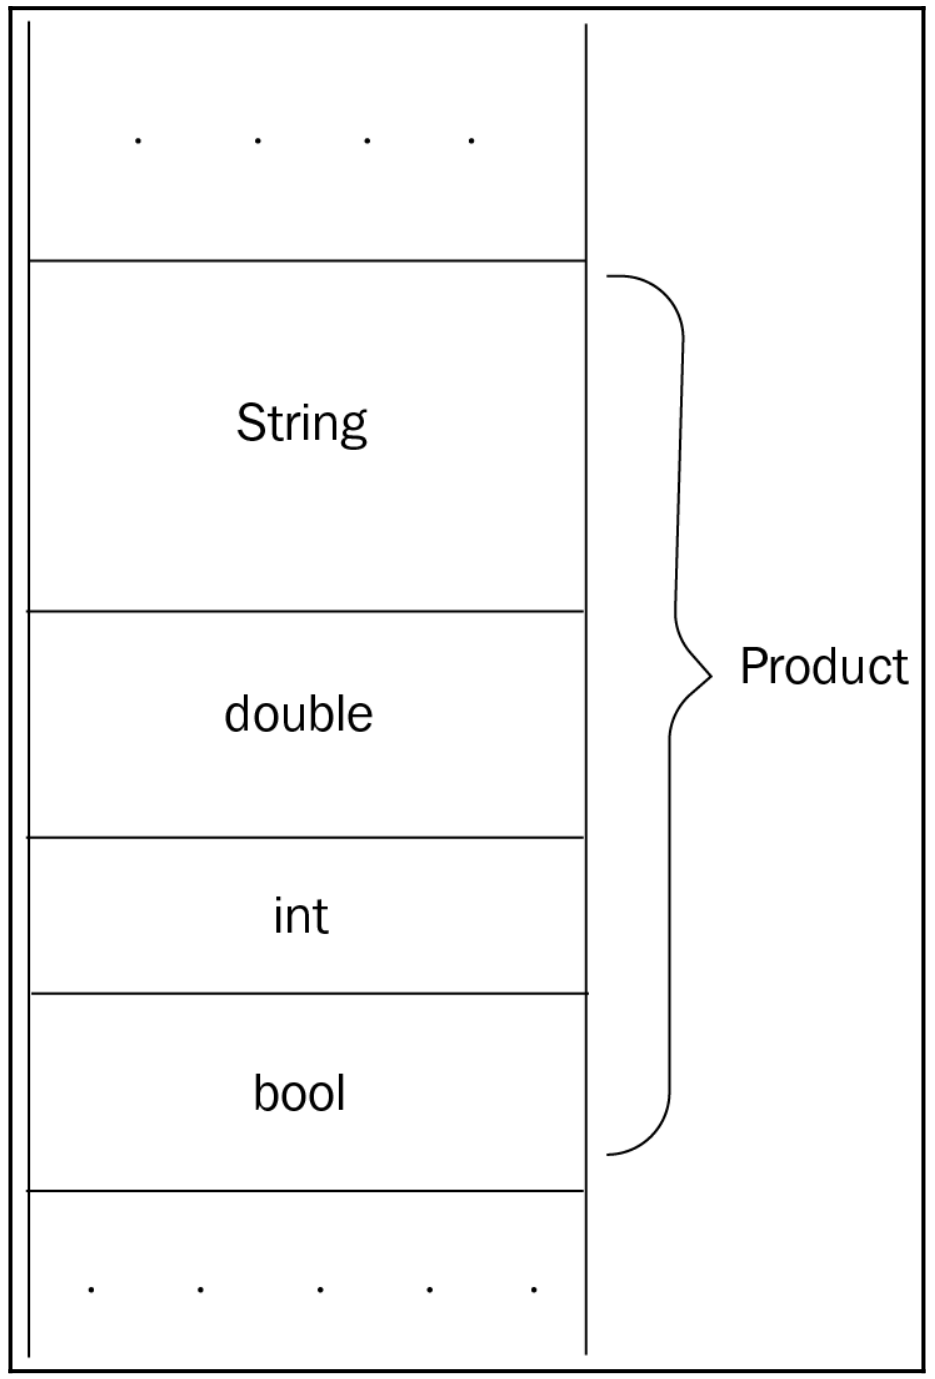
\includegraphics[width=0.4\textwidth]{content/Section-1/Chapter-3/1}
\end{center}

声明Product对象需要在内存中使用sizeof(Product)空间,而声明对象的指针或引用需要存储地址所需的空间(通常为4或8个字节)。参见以下代码块:\par

\begin{lstlisting}[caption={}]
Product book;
Product tshirt;
Product* ptr = &book;
Product& ref = tshirt;
\end{lstlisting}

上面的代码描述如下: \par

\begin{center}
	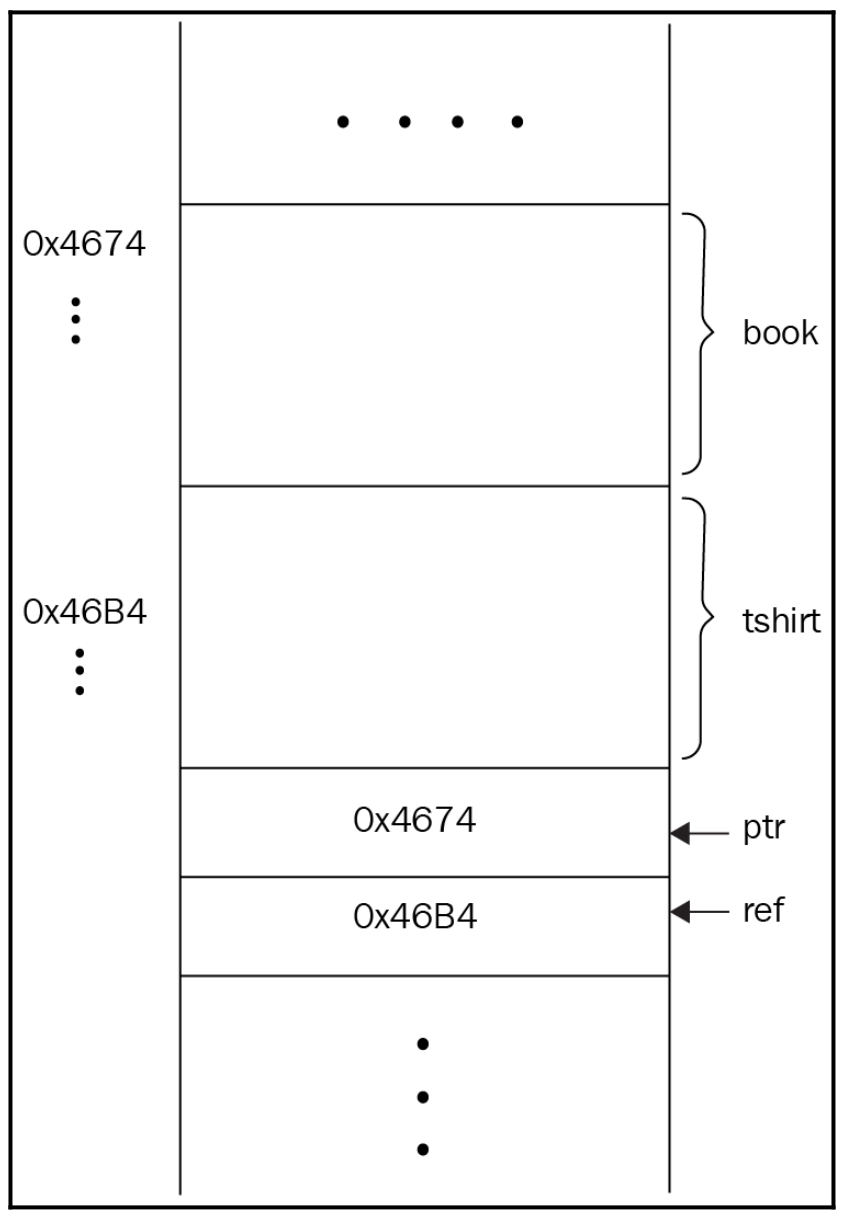
\includegraphics[width=0.4\textwidth]{content/Section-1/Chapter-3/2}
\end{center}

从Product对象在内存中占用的空间开始。可以计算Product对象的大小,并将其成员变量的大小加起来。布尔变量的大小是1字节。C++标准中没有指定double类型或int类型的确切大小。在64位机器中,double变量通常需要8个字节,而int变量需要4个字节。 \par
std::string的实现没有在标准中指定,所以它的大小取决于标准库的实现。string存储一个指向字符数组的指针,也可以存储已分配字符的数量,可在调用size()时有效地返回该指针。string的一些实现需要8、24或32个字节的内存,但在我们的示例中由24个字节。Product对象的大小如下:\par
	\texttt{24 (std::string) + 8 (double) + 4 (int) + 1 (bool) = 37 bytes.} \par

\noindent\textbf{}\ \par
打印Product的大小会输出一个不同的值: \par
	\texttt{std::cout << sizeof(Product);} \par
	
\noindent\textbf{}\ \par
输出的是40,而不是计算的37。冗余字节背后的原因是结构体的填充,编译器使用这种技术来优化对对象的各个成员的访问。中央处理器(CPU)以固定大小的字读取内存。字的大小由CPU定义(通常是32位或64位长)。如果从一个字对齐的地址开始,中央处理器则能够访问数据。例如,Product的布尔数据成员需要1字节的内存,可以放在rating之后。编译器会对数据进行对齐,从而实现更快的访问。我们假设单词的大小是4个字节,如果变量从一个能被4整除的地址开始,CPU将不需要执行冗余步骤就可以访问这个变量。编译器在前面的结构体中添加额外的字节,使成员地址与边界地址对齐。

\noindent\textbf{}\ \par
\textbf{对象的高层细节} \ \par
我们把对象当作代表抽象结果的实体来处理。我们已经提到了观察者,即基于问题域定义对象的开发者,定义它的方式代表了抽象的过程。我们以电子商务市场及其产品为例,两个不同的编程团队可能对同一产品有不同的看法。实现网站的团队关心对象的属性,这对网站访问者来说是必不可少的买家。我们前面在Product结构中显示的属性大多是为网站访问者准备的,如销售价格、产品评级等。实现网站的开发者需要接触问题域,并验证定义Product对象所必需的属性。 \par
实现帮助管理仓库中产品的团队关心对象的属性,这些属性在产品放置、质量控制和装运方面必不可少。这个团队实际上不应该关心产品的评级,甚至价格。这个团队主要关心产品的重量、尺寸和条件。下图显示了感兴趣的属性:\par

\begin{center}
	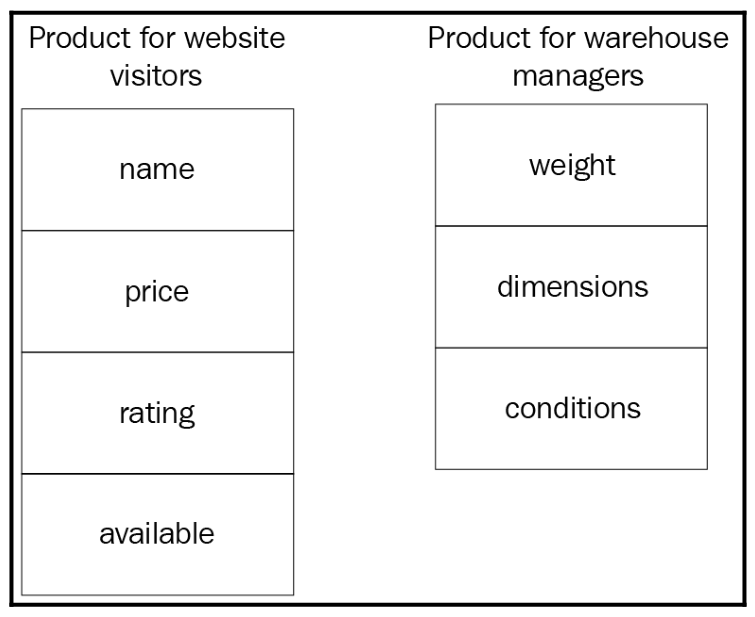
\includegraphics[width=0.4\textwidth]{content/Section-1/Chapter-3/3}
\end{center}

开发者在开始项目时应该做的第一件事,是分析问题并收集需求。换句话说,他们应该熟悉问题领域并定义项目需求。分析的过程导致定义对象及其类型,例如:前面讨论的Product。为了从分析中得到适当的结果,应该在对象中思考,考虑对象的三个主要属性:状态、行为和特性。\par

\noindent\textbf{}\ \par
\textbf{状态} \ \par
每个对象都有一个状态,可能与其他对象的状态不同。我们已经介绍了产品结构,它表示物理(或数字)产品的抽象。Product对象的所有成员共同表示对象的状态,例如:Product包含成员available,这是一个布尔值,如果产品有库存,则为true。成员变量的值定义了对象的状态。如果给对象成员赋值,它的状态也会改变: \par

\begin{lstlisting}[caption={}]
Product cpp_book; // declaring the object
...
// changing the state of the object cpp_book
cpp_book.available = true;
cpp_book.rating = 5;
\end{lstlisting}

对象的状态是它所有属性和值的集合。 \par

\noindent\textbf{}\ \par
\textbf{特性} \ \par
特性是区分一个物体与另一个物体的属性。即使我们试图声明两个物理上不可区分的对象,它们的变量仍然有不同的名称,即不同的标识符: \par

\begin{lstlisting}[caption={}]
Product book1;
book1.rating = 4;
book1.name = "Book";
Product book2;
book2.rating = 4;
book2.name = "Book";
\end{lstlisting}

前面示例中的对象具有相同的状态,但不同之处在于我们引用它们的名称,即book1和book2。假设我们能够以某种方式创建具有相同名称的对象,如下面的代码所示: \par

\begin{lstlisting}[caption={}]
Product prod;
Product prod; // won't compile, but still "what if?"
\end{lstlisting}

如果是这样可行,它们会在内存中有不同的地址: \par

\begin{center}
	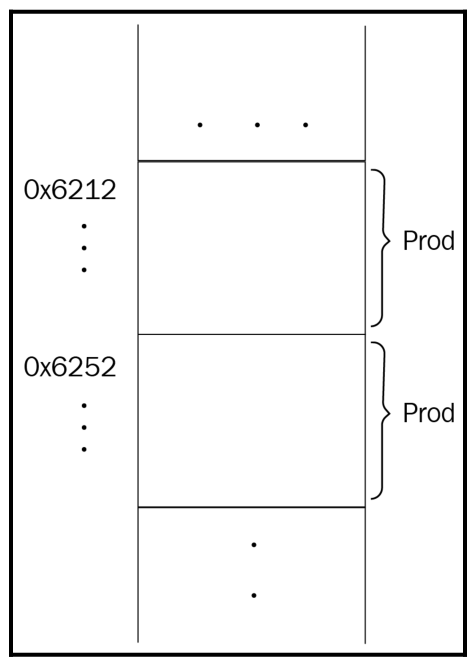
\includegraphics[width=0.4\textwidth]{content/Section-1/Chapter-3/4}
\end{center}

特性是对象的一个基本属性,也是我们不能创建空对象的原因之一,如下所示:\par

\begin{lstlisting}[caption={}]
struct Empty {};
int main() {
	Empty e;
	std::cout << sizeof(e);
}
\end{lstlisting}

前面的代码不会像预期的那样输出0。标准中没有指定空对象的大小,编译器开发人员倾向于为这些对象分配1个字节,可能也会遇到4或8个字节。两个或两个以上的Empty实例在内存中应该有不同的地址,因此编译器必须确保对象将占用至少1个字节的内存。 \par

\noindent\textbf{}\ \par
\textbf{行为} \ \par
前面的例子中,我们将5和4分别赋值给rating成员变量,所以很容易因为给对象赋值无效而出错,比如:\par

\begin{lstlisting}[caption={}]
cpp_book.rating = -12;
\end{lstlisting}

-12对于产品的评级来说是无效的,否则会让用户感到困惑。我们可以通过提供setter函数来控制对象改变的行为: \par

\begin{lstlisting}[caption={}]
void set_rating(Product* p, int r) {
	if (r >= 1 && r <= 5) {
		p->rating = r;
	}
	// otherwise ignore
}
...
set_rating(&cpp_book, -12); // won't change the state
\end{lstlisting}

对象对的操作和相应源自于其他对象的请求。请求是通过函数调用来执行的,否则称为消息:一个对象将消息传递给另一个对象。前面的示例中,将相应的set\underline{ }rating消息传递给cpp\underline{ }book对象。本例中,我们假设从main()调用函数,它实际上根本不表示任何对象。我们可以说它是全局对象,不过C++中没有这样的实体可以操作main()函数的对象。 \par
我们从概念上而不是物理上区分对象。面向对象编程的一些概念的物理实现并不是标准化的,因此我们可以将Product结构命名为一个类,并声明cpp\underline{ }book是Product的一个实例,并且具有一个名为set\underline{ }rating()的成员函数。C++实现做了同样的事情:提供了语法上的结构(类、可见性修饰符、继承等等),并将它们转换为简单的结构,使用全局函数,如前面示例中的set\underline{ }rating()。现在,让我们深入研究C++对象模型的细节。 \par

\noindent\textbf{}\ \par
\textbf{模仿类} \ \par
struct允许我们对变量进行分组、命名和创建对象。类的思想是在对象中包含相应的操作,对数据和特定数据的操作进行分组。例如,对于Product类型的对象,直接调用set\underline{}rating()函数就很自然的,而不是使用全局函数,通过指针接受Product对象进行修改。然而,由于在C语言中使用结构体,不能使用成员函数。为了模拟使用C结构的类,我们必须将使用Product对象的函数声明为全局函数,如下面代码所示:\par

\begin{lstlisting}[caption={}]
struct Product {
	std::string name;
	double price;
	int rating;
	bool available;
};
void initialize(Product* p) {
	p->price = 0.0;
	p->rating = 0;
	p->available = false;
}
void set_name(Product* p, const std::string& name) {
	p->name = name;
}
std::string get_name(Product* p) {
	return p->name;
}
void set_price(Product* p, double price) {
	if (price < 0 || price > 9999.42) return;
	p->price = price;
}
double get_price(Product* p) {
	return p->price;
}
// code omitted for brevity
\end{lstlisting}

要将结构体作为类使用,我们应该按正确的顺序调用函数。例如,使用正确的初始化默认值对对象进行初始化,所以必须调用initialize()函数:\par

\begin{lstlisting}[caption={}]
int main() {
	Product cpp_book;
	initialize(&cpp_book);
	set_name(&cpp_book, "Mastering C++ Programming");
	std::cout << "Book title is: " << get_name(&cpp_book);
	// ...
}
\end{lstlisting}

这似乎是可行的,但如果添加了新类型,代码很快就会变得杂乱无章。例如:Warehouse,用于跟踪产品仓库的结构体: \par

\begin{lstlisting}[caption={}]
struct Warehouse {
	Product* products;
	int capacity;
	int size;
};
void initialize_warehouse(Warehouse* w) {
	w->capacity = 1000;
	w->size = 0;
	w->products = new Product[w->capacity];
	for (int ix = 0; ix < w->capacity; ++ix) {
		initialize(&w->products[ix]); // initialize each Product object
	}
}
void set_size(int size) { ... }
// code omitted for brevity
\end{lstlisting}

第一个明显的问题是函数的命名。我们必须为仓库initialize\underline{ }warehouse的初始化函数命名,以避免与已经声明的产品initialize()函数发生冲突。我们可以考虑为产品类型重命名函数,以避免将来可能发生的冲突。接下来是混乱的函数,我们有一堆全局函数,随着我们添加新类型,它们的数量会增加。如果我们添加一些类型层次结构,则更加难以管理。\par
尽管编译器倾向于将类转换为具有全局函数的结构,但正如前面所示,C++和其他高级编程语言解决了这些问题,引入了平滑机制的类,将它们组织到层次结构中。从概念上讲,关键字(类、公共或私有)和机制(继承和多态性)可以方便地让开发人员组织代码。 \par

\noindent\textbf{}\ \par
\textbf{使用类} \ \par
处理对象时,类使事情变得容易得多。完成OOP中最简单的必要工作:它们将数据与用于操作数据的函数结合起来。我们用类重写Product结构体的例子: \par

\begin{lstlisting}[caption={}]
class Product {
public:
	Product() = default; // default constructor
	Product(const Product&); // copy constructor
	Product(Product&&); // move constructor
	Product& operator=(const Product&) = default;
	Product& operator=(Product&&) = default;
	// destructor is not declared, should be generated by the compiler
	
public:
	void set_name(const std::string&);
	std::string name() const;
	void set_availability(bool);
	bool available() const;
	// code omitted for brevity
	
private:
	std::string name_;
	double price_;
	int rating_;
	bool available_;
};

std::ostream& operator<<(std::ostream&, const Product&);
std::istream& operator>>(std::istream&, Product&);
\end{lstlisting}

类声明似乎更有组织,尽管它公开的函数比定义类似结构时使用的函数更多。我们应该这样来说明这个类: \par

\begin{center}
	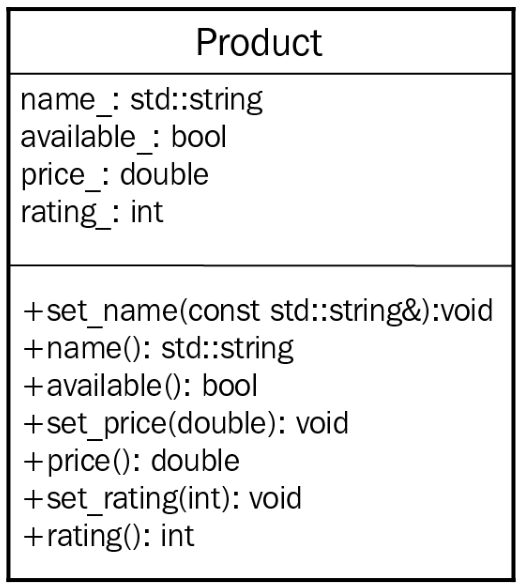
\includegraphics[width=0.4\textwidth]{content/Section-1/Chapter-3/5}
\end{center}

前面的图像有些特殊,它有组织的节,函数名之前的符号等。这类图称为统一建模语言(UML)类图。UML是一种标准化阐明类及其关系的过程的方法。第一部分是类的名称(用粗体表示),接下来是成员变量部分,然后是成员函数部分。函数名前面的+(加号)表示该函数是公共的。成员变量通常是私有的,但如果需要强调这一点,可以使用-(减号)。我们可以通过简单地说明类来省略所有细节,如下面的UML图所示: \par

\begin{center}
	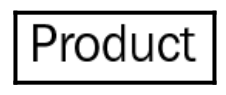
\includegraphics[width=0.1\textwidth]{content/Section-1/Chapter-3/6}
\end{center}

我们将在本书中使用UML图,并根据需要引入新的图类型。在处理初始化、复制、移动、默认和删除函数。在重载操作符之前,先清理一些东西。 \par

\noindent\textbf{}\ \par
\textbf{从编译器的角度来看类} \ \par
首先,不管前面的类与前面介绍的结构体相比有多么怪异,编译器都会将其翻译成以下代码(简单起见,稍微修改了下):\par

\begin{lstlisting}[caption={}]
struct Product {
	std::string name_;
	bool available_;
	double price_;
	int rating_;
};

// we forced the compiler to generate the default constructor
void Product_constructor(Product&);
void Product_copy_constructor(Product& this, const Product&);
void Product_move_constructor(Product& this, Product&&);

// default implementation
Product& operator=(Product& this, const Product&);

// default implementation
Product& operator=(Product& this, Product&&);
void Product_set_name(const std::string&);

// takes const because the method was declared as const
std::string Product_name(const Product& this);
void Product_set_availability(Product& this, bool b);
bool Product_availability(const Product& this);
std::ostream& operator<<(std::ostream&, const Product&);
std::istream& operator>>(std::istream&, Product&);
\end{lstlisting}

基本上,编译器生成的代码与我们前面介绍的代码相同,可以使用一个简单的结构来模拟类行为。尽管编译器在实现C++对象模型的技术和方法上各不相同,但上面的例子是编译器开发人员常用的方法。它平衡了访问对象成员(包括成员函数)的空间和时间效率。 \par
接下来,们应该考虑编译器如何通过扩充和修改代码来编辑我们的代码。下面的代码声明了全局的create\underline{ }apple()函数,该函数创建并返回一个Product对象,该对象的值特定为apple。还在main()函数中声明了一个book对象: \par

\begin{lstlisting}[caption={}]
Product create_apple() {
	Product apple;
	apple.set_name("Red apple");
	apple.set_price("0.2");
	apple.set_rating(5);
	apple.set_available(true);
	return apple;
}

int main() {
	Product red_apple = create_apple();
	Product book;
	Product* ptr = &book;
	ptr->set_name("Alice in Wonderland");
	ptr->set_price(6.80);
	std::cout << "I'm reading " << book.name()
	<< " and I bought an apple for " << red_apple.price()
	<< std::endl;
}
\end{lstlisting}

我们已经知道,编译器修改类,将其转换为结构体,并将成员函数移动到全局作用域,每个成员函数都将类的引用(或指针)作为其第一个形参。为了在客户端代码中支持这些修改,还应该修改对象的所有访问方式。 \par

\hspace*{\fill} \\ %插入空行

\includegraphics[width=0.05\textwidth]{images/tip}
声明或已声明的类对象的代码称为客户端代码。\par
\noindent\textbf{}\ \par

下面是我们如何假设编译器修改了前面的代码(使用这个词是试图引入编译器抽象,而不是特定的某个编译器):\par

\begin{lstlisting}[caption={}]
void create_apple(Product& apple) {
	Product_set_name(apple, "Red apple");
	Product_set_price(apple, 0.2);
	Product_set_rating(apple, 5);
	Product_set_available(apple, true);
	return;
}
int main() {
	Product red_apple;
	Product_constructor(red_apple);
	create_apple(red_apple);
	Product book;
	Product* ptr;
	Product_constructor(book);
	Product_set_name(*ptr, "Alice in Wonderland");
	Product_set_price(*ptr, 6.80);
	std::ostream os = operator<<(std::cout, "I'm reading ");
	os = operator<<(os, Product_name(book));
	os = operator<<(os, " and I bought an apple for ");
	os = operator<<(os, Product_price(red_apple));
	operator<<(os, std::endl);
	// destructor calls are skipped because the compiler
	// will remove them as empty functions to optimize the code
	// Product_destructor(book);
	// Product_destructor(red_apple);
}
\end{lstlisting}

编译器还优化了对create\underline{ }apple()函数的调用,以避免临时创建对象。我们将在本章后面讨论编译器生成的临时文件。\par

\noindent\textbf{}\ \par
\textbf{初始化和销毁} \ \par
如前所述,对象的创建需要两个步骤:内存分配和初始化。内存分配是对象声明的结果,C++不关心变量的初始化分配内存(不管是自动的还是手动的)。实际的初始化应该由开发者来完成,这就是为什么首先要有一个构造函数。 \par
析构函数遵循同样的逻辑。如果忽略默认构造函数或析构函数的声明,编译器应该隐式生成它们,如果它们为空,编译器也会删除它们(消除对空函数的冗余调用)。如果声明了任何带形参的构造函数,包括复制构造函数,编译器将不会生成默认构造函数。我们可以强制编译器隐式生成默认构造函数: \par

\begin{lstlisting}[caption={}]
class Product {
	public:
	Product() = default;
	// ...
};
\end{lstlisting}

也可以使用delete说明符来强制它不生成编译器,如下所示:\par

\begin{lstlisting}[caption={}]
class Product {
	public:
	Product() = delete;
	// ...
};
\end{lstlisting}

这将禁止默认初始化的对象声明,即\texttt{Product p;}编译会报错。 \par

\hspace*{\fill} \\ %插入空行

\includegraphics[width=0.05\textwidth]{images/tip}
析构函数的调用顺序与对象声明的顺序相反,因为自动内存分配是由堆栈管理的,堆栈是遵循后进先出(LIFO)规则的数据结构。 \par
\noindent\textbf{}\ \par

对象在创建时进行初始化,销毁通常发生在对象不再可访问时。当在堆上分配对象时,后者可能比较棘手。看看下面的代码,在不同的作用域和内存段中声明了四个Product对象: \par

\begin{lstlisting}[caption={}]
static Product global_prod; // #1
Product* foo() {
	Product* heap_prod = new Product(); // #4
	heap_prod->name = "Sample";
	return heap_prod;
}
int main() {
	Product stack_prod; // #2
	if (true) {
		Product tmp; // #3
		tmp.rating = 3;
	}
	stack_prod.price = 4.2;
	foo();
}
\end{lstlisting}

global\underline{ }prod有一个静态的存储期,并且放置在程序的global/static部分,在main()调用前初始化。main()开始时,在堆栈上分配stack\underline{ }prod,并在main()结束时销毁(函数的右花括号被认为是它的结束)。尽管条件表达式看起来很奇怪,但它是表达作用域的好方法。\par
tmp对象也在堆栈上分配,但是它的存储期限制在声明的范围内:当离开if块时,将自动销毁。这就是为什么栈上的变量具有自动存储期。最后,调用foo()函时,声明了stack\underline{ }prod指针,该指针指向在堆上分配的Product对象的地址。 \par
前面的代码有内存泄漏,当执行到达foo()的末尾时,stack\underline{ }prod指针(本身有一个自动存储其)将销毁,而在堆上分配的对象不会受到影响。不要混淆指针和它所指向的实际对象:指针只包含对象的值,但不代表对象。 \par

\hspace*{\fill} \\ %插入空行

\includegraphics[width=0.05\textwidth]{images/tip}
不要忘记释放在堆上动态分配的内存,可以手动调用delete操作符,也可以使用智能指针。智能指针将在第5章讨论。 \par
\noindent\textbf{}\ \par

函数结束时,分配给堆栈的参数和局部变量的内存将被释放。当程序结束时,main()函数结束后,global\underline{ }prod将销毁。析构函数将在对象即将销毁时调用。 \par

\noindent\textbf{}\ \par
\textbf{复制对象} \ \par
有两种类型的复制:对象的深度复制和浅层复制。语言允许我们使用复制构造函数和赋值操作符,管理对象的复制初始化和赋值。这对于程序员来说是一个必要的特性,这样我们就可以控制复制语义。看看下面的例子: \par

\begin{lstlisting}[caption={}]
Product p1;
Product p2;
p2.set_price(4.2);
p1 = p2; // p1 now has the same price
Product p3 = p2; // p3 has the same price
\end{lstlisting}

\texttt{p1 = p2;}是对赋值操作符的调用,而最后一行是对复制构造函数的调用。等号不应该让开发者混淆它是赋值调用还是复制构造函数。每次看到声明后面跟着赋值,就当作复制构造。这适用于新的初始化器语法(\texttt{Product p3\{p2\};})。 \par

编译器将生成以下代码: \par

\begin{lstlisting}[caption={}]
Product p1;
Product p2;
Product_set_price(p2, 4.2);
operator=(p1, p2);
Product p3;
Product_copy_constructor(p3, p2);
\end{lstlisting}

复制构造函数(和赋值操作符)的默认实现按成员方式复制对象,如下图所示: \par

\begin{center}
	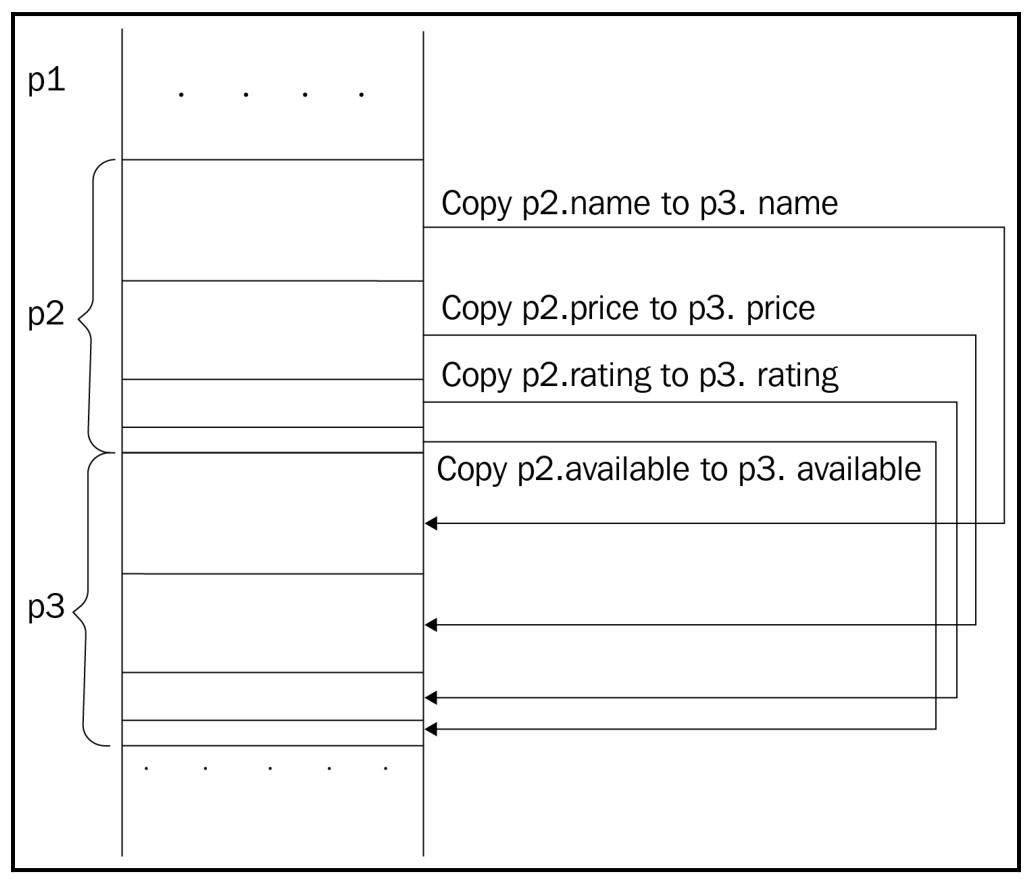
\includegraphics[width=0.4\textwidth]{content/Section-1/Chapter-3/7}
\end{center}

如果成员副本产生无效副本,则需要自定义实现。例如,考虑以下仓库对象的副本: \par

\begin{lstlisting}[caption={}]
class Warehouse {
public:
	Warehouse()
	: size_{0}, capacity_{1000}, products_{nullptr}
	{
		products_ = new Products[capacity_];
	}
	~Warehouse() {
		delete [] products_;
	}

public:
	void add_product(const Product& p) {
		if (size_ == capacity_) { /* resize */ }
		products_[size_++] = p;
	}
	// other functions omitted for brevity
	
private:
	int size_;
	int capacity_;
	Product* products_;
};

int main() {
	Warehouse w1;
	Product book;
	Product apple;
	// ...assign values to products (omitted for brevity)
	w1.add_product(book);
	Warehouse w2 = w1; // copy
	w2.add_product(apple);
	// something somewhere went wrong...
}
\end{lstlisting}

前面的代码声明了两个Warehouse对象,然后将两个不同的产品添加到仓库中。虽然这个例子有点不自然,但它展示了默认复制实现的危险性。下面的插图向我们展示了代码中出错的地方: \par

\begin{center}
	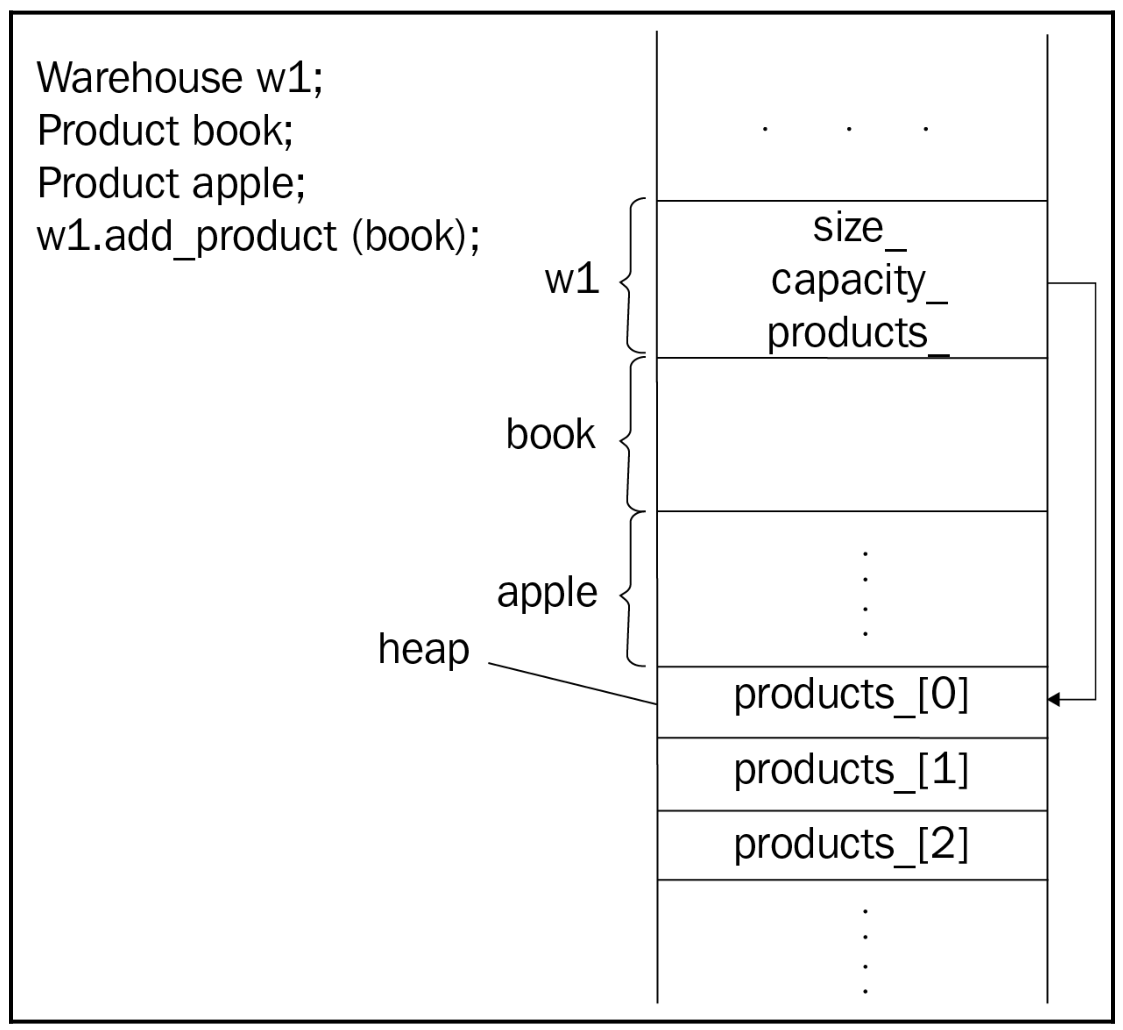
\includegraphics[width=0.4\textwidth]{content/Section-1/Chapter-3/8}
\end{center}

将w1分配给w2会导致如下结构: \par

\begin{center}
	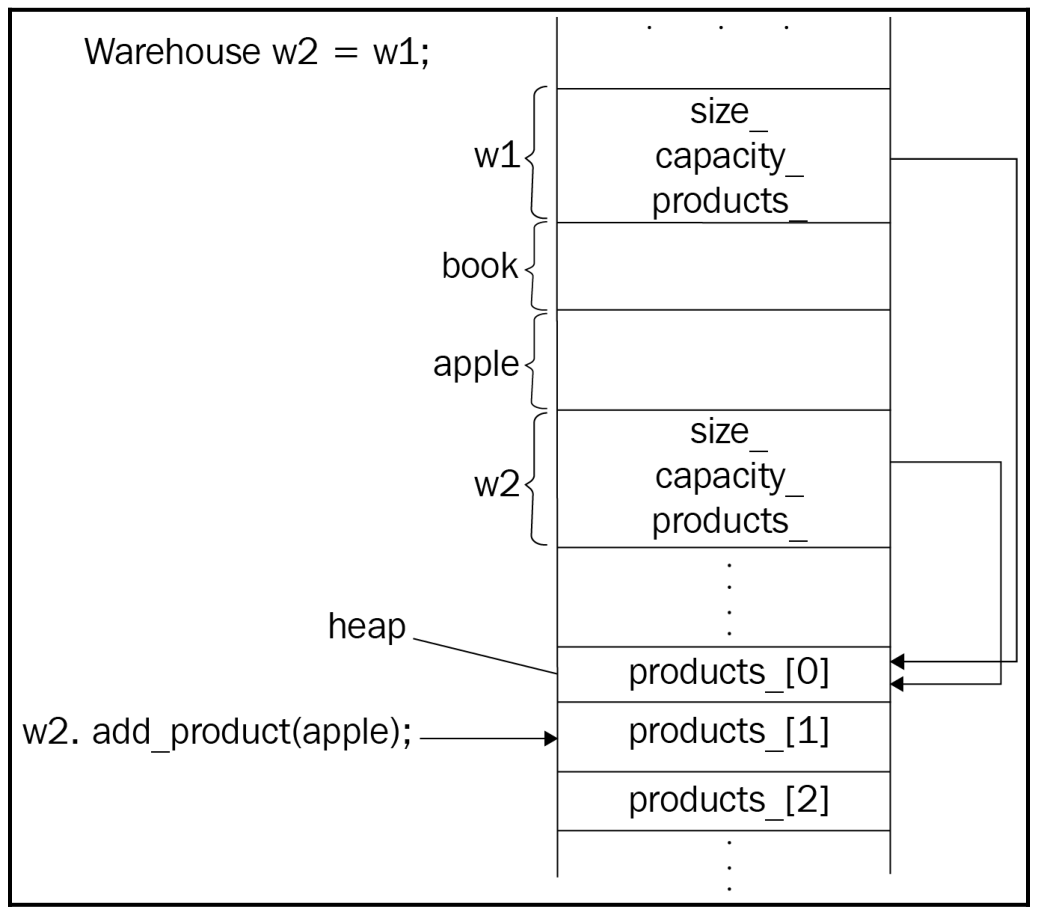
\includegraphics[width=0.4\textwidth]{content/Section-1/Chapter-3/9}
\end{center}

默认实现只是简单地将w1的每个成员复制到w2。复制之后,w1和w2的products\underline{ }成员都指向堆上的相同位置。当我们向w2添加一个新产品时,w1所指向的数组将受到影响。这是一个逻辑错误,可能会导致程序中未定义的行为。我们需要的是深复制的而不是浅复制,需要实际创建一个包含w1数组副本的新产品数组。 \par
复制构造函数和赋值操作符的自定义实现解决了浅复制的问题: \par

\begin{lstlisting}[caption={}]
class Warehouse {
public:
	// ...
	Warehouse(const Warehouse& rhs) {
		size_ = rhs.size_;
		capacity_ = rhs.capacity_;
		products_ = new Product[capacity_];
		for (int ix = 0; ix < size_; ++ix) {
			products_[ix] = rhs.products_[ix];
		}
	}
	// code omitted for brevity
};
\end{lstlisting}

复制构造函数的自定义实现创建了新数组。然后,逐个复制源对象的数组元素,这样就消除了product\underline{ }指针指向错误内存地址的可能。换句话说,我们通过创建新数组实现了对仓库对象的深复制。 \par

\noindent\textbf{}\ \par
\textbf{移动对象} \ \par
代码中到处都是临时对象。大多数情况下,他们都需要让代码按照预期工作。例如,当将两个对象相加时,会创建一个临时对象来保存操作符+的返回值: \par

\begin{lstlisting}[caption={}]
Warehouse small;
Warehouse mid;
// ... some data inserted into the small and mid objects
Warehouse large{small + mid}; // operator+(small, mid)
\end{lstlisting}

让我们来看看Warehouse对象的全局操作符+的实现: \par

\begin{lstlisting}[caption={}]
// considering declared as friend in the Warehouse class
Warehouse operator+(const Warehouse& a, const Warehouse& b) {
	Warehouse sum; // temporary
	sum.size_ = a.size_ + b.size_;
	sum.capacity_ = a.capacity_ + b.capacity_;
	sum.products_ = new Product[sum.capacity_];
	
	for (int ix = 0; ix < a.size_; ++ix) { sum.products_[ix] =
		a.products_[ix]; }
	for (int ix = 0; ix < b.size_; ++ix) { sum.products_[a.size_ + ix] =
		b.products_[ix]; }
	
	return sum;
}
\end{lstlisting}

前面的实现声明了一个临时对象,并在用必要的数据填充它后返回它。前面例子中的调用可以翻译成以下形式: \par

\begin{lstlisting}[caption={}]
Warehouse small;
Warehouse mid;
// ... some data inserted into the small and mid objects
Warehouse tmp{operator+(small, mid)};
Warehouse large;
Warehouse_copy_constructor(large, tmp);
__destroy_temporary(tmp);
\end{lstlisting}

C++11中引入的移动语义,允许通过将返回值移动到Warehouse对象中,从而跳过临时变量的创建。要做到这一点,我们应该为仓库声明一个移动构造函数,它可以区分临时对象并有效地处理它们: \par

\begin{lstlisting}[caption={}]
class Warehouse {
public:
	Warehouse(); // default constructor
	Warehouse(const Warehouse&); // copy constructor
	Warehouse(Warehouse&&); // move constructor
	// code omitted for brevity
};
\end{lstlisting}

移动构造函数的形参是右值引用(\&\&). \par

\noindent\textbf{}\ \par
\textbf{左值引用} \ \par
理解为什么引入右值引用之前,让我们先弄清楚左值、引用和左值引用。当一个变量是左值时,它可以寻址,可以指向,并且它有一个作用域存储周期: \par

\begin{lstlisting}[caption={}]
double pi{3.14}; // lvalue
int x{42}; // lvalue
int y{x}; // lvalue
int& ref{x}; // lvalue-reference
\end{lstlisting}

ref是左值引用,可以视为const指针的变量同义词: \par

\begin{lstlisting}[caption={}]
int * const ref = &x;
\end{lstlisting}

除了通过引用修改对象的能力之外,我们还通过引用将重对象传递给函数,以优化和避免冗余的对象副本。例如,仓库的操作符+通过引用传入两个对象,这时是复制对象的地址,而不是完整的对象。 \par
左值引用在函数调用方面优化了代码,但是为了优化临时代码,我们应该转向右值引用。 \par

\noindent\textbf{}\ \par
\textbf{右值引用} \ \par
不能将左值引用绑定到临时对象。下面的代码就无法进行编译: \par

\begin{lstlisting}[caption={}]
int get_it() {
	int it{42};
	return it;
}
...
int& impossible{get_it()}; // compile error
\end{lstlisting}

我们需要声明一个右值引用,以便能够绑定到临时对象(包括字面字值): \par

\begin{lstlisting}[caption={}]
int&& possible{get_it()};
\end{lstlisting}

右值引用允许我们尽可能地跳过临时对象的生成。例如,将结果作为右值引用的函数,通过消除临时对象的方式运行得更快: \par

\begin{lstlisting}[caption={}]
void do_something(int&& val) {
	// do something with the val
}
// the return value of the get_it is moved to do_something rather than
copied
do_something(get_it());
\end{lstlisting}

想象移动的效果,想象前面的代码将转译成以下代码(只是为了体现移动的完整概念):\par

\begin{lstlisting}[caption={}]
int val;
void get_it() {
	val = 42;
}
void do_something() {
	// do something with the val
}
do_something();
\end{lstlisting}

在引入移动之前,前面的代码看起来是这样的(经过编译器优化):\par

\begin{lstlisting}[caption={}]
int tmp;
void get_it() {
	tmp = 42;
}
void do_something(int val) {
	// do something with the val
}
do_something(tmp);
\end{lstlisting}

当输入参数表示右值时,移动构造函数和移动操作符=()具有复制的效果,而不需要实际执行复制。这就是为什么我们应该在类中实现这些新函数的原因:这样就可以在任何有意义的地方优化代码。移动构造函数可以获取源对象,而不是复制它。代码如下所示: \par

\begin{lstlisting}[caption={}]
class Warehouse {
public:
	// constructors omitted for brevity
	Warehouse(Warehouse&& src)
	: size_{src.size_},
	capacity_{src.capacity_},
	products_{src.products_}
	{
		src.size_ = 0;
		src.capacity_ = 0;
		src.products_ = nullptr;
	}
};
\end{lstlisting}

不创建一个capacity\underline{ }大小的新数组,然后复制products\underline{ }数组的每个元素了,这次只是获取了指向该数组的指针。我们知道src对象是右值,它很快就会销毁,这意味着析构函数将调用,析构函数将删除已分配的数组。现在,将新创建的Warehouse对象指向已分配的数组,这就是为什么不能让析构函数删除源数组的原因。我们将nullptr赋值给它,以确保析构函数跳过已分配的对象。因此,下面的代码将因为移动构造函数得到了优化: \par

\begin{lstlisting}[caption={}]
Warehouse large = small + mid;
\end{lstlisting}

+操作符的结果是移动而不是复制。请看下面的图表:\par

\begin{center}
	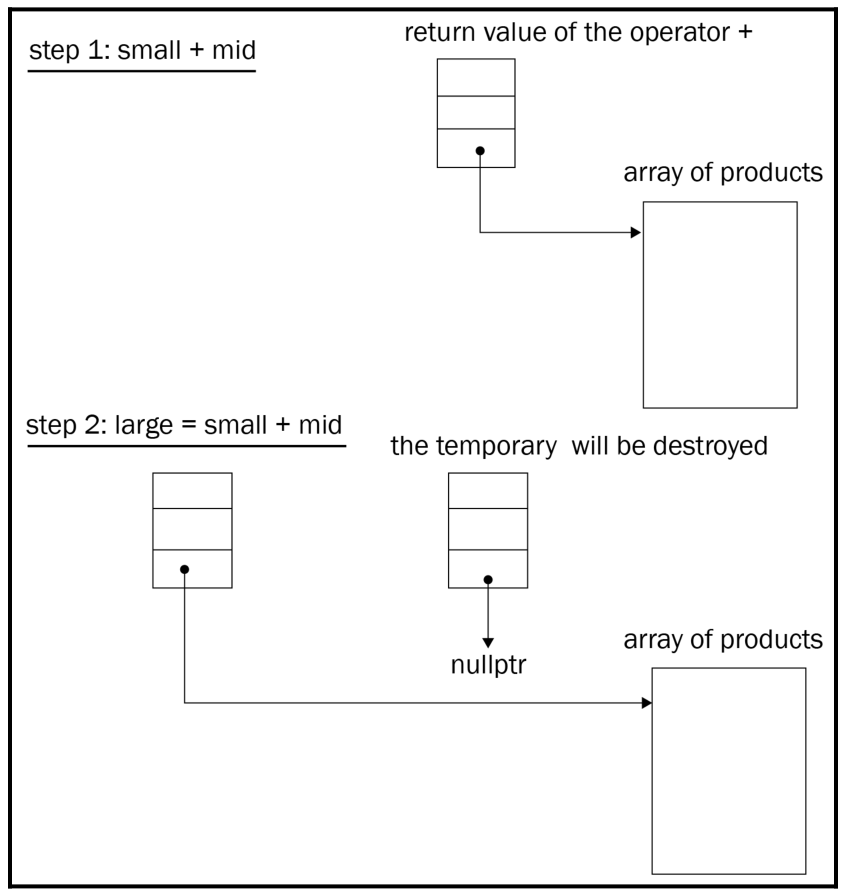
\includegraphics[width=0.4\textwidth]{content/Section-1/Chapter-3/10}
\end{center}

\noindent\textbf{}\ \par
\textbf{操作符重载的注意事项} \ \par
C++为自定义类型的重载操作符提供了强大的机制,使用+操作符计算两个对象的和要比调用成员函数好得多。调用成员函数还需要在调用它之前记住它的名称。它可能是add, calculatessum, calculate\underline{ }sum或其他。操作符重载允许在类设计中采用一致的方法,重载操作符会增加代码中不必要的冗长。下面的代码片段重载了一组比较运算符,以及Money类的加减运算符:\par

\begin{lstlisting}[caption={}]
constexpr bool operator<(const Money& a, const Money& b) {
	return a.value_ < b.value_;
}
constexpr bool operator==(const Money& a, const Money& b) {
	return a.value_ == b.value_;
}
constexpr bool operator<=(const Money& a, const Money& b) {
	return a.value_ <= b.value_;
}
constexpr bool operator!=(const Money& a, const Money& b) {
	return !(a == b);
}
constexpr bool operator>(const Money& a, const Money& b) {
	return !(a <= b);
}
constexpr bool operator>=(const Money& a, const Money& b) {
	return !(a < b);
}
constexpr Money operator+(const Money& a, const Money& b) {
	return Money{a.value_ + b.value_};
}
constexpr Money operator-(const Money& a, const Money& b) {
	return Money{a.value_ - b.value_};
}
\end{lstlisting}

前面的大多数函数都直接访问Money实例的value成员。为了让它起作用,我们应该宣布他们为Money的朋友。以下是Money的类: \par

\begin{lstlisting}[caption={}]
class Money
{
public:
	Money() {}
	explicit Money(double v) : value_{v} {}
	// construction/destruction functions omitted for brevity
public:
	friend constexpr bool operator<(const Money&, const Money&);
	friend constexpr bool operator==(const Money&, const Money&);
	friend constexpr bool operator<=(const Money&, const Money&);
	friend constexpr bool operator!=(const Money&, const Money&);
	friend constexpr bool operator>(const Money&, const Money&);
	friend constexpr bool operator>=(const Money&, const Money&);
	friend constexpr bool operator+(const Money&, const Money&);
	friend constexpr bool operator-(const Money&, const Money&);
private:
	double value_;
};
\end{lstlisting}

这类看起来怪极了。C++20介绍了spaceship操作符,它允许我们跳过比较操作符的定义。<=>,也称为三向比较操作符,请求编译器生成关系操作符。对于Money类,可以使用默认的<=>,如下所示: \par

\begin{lstlisting}[caption={}]
class Money
{
	// code omitted for brevity
	friend auto operator<=>(const Money&, const Money&) = default;
};
\end{lstlisting}

编译器将生成==、!=、<、>、<=、>=操作符。spaceship操作符减少了操作符的冗余定义,并为生成的所有操作符提供了一种实现通用方法。在为spaceship操作符实现自定义行为时,我们应该注意操作符的返回值类型。它可以是下列之一: \par

\begin{itemize}
	\item \texttt{std::strong\underline{ }ordering}
	\item \texttt{std::weak\underline{ }ordering}
	\item \texttt{std::partial\underline{ }ordering}
	\item \texttt{std::strong\underline{ }equality}
	\item \texttt{std::weak\underline{ }equality}
\end{itemize}

它们都是在<compare>头文件中定义的。编译器根据三向操作符的返回类型生成操作符。\par

\noindent\textbf{}\ \par
\textbf{封装和公共接口} \ \par
封装是面向对象编程中的关键概念,允许对客户端代码隐藏对象的实现细节。以电脑键盘为例,它有字母、数字和符号的键,如果我们按下这些键,就会起作用。键盘的使用简单直观,隐藏了许多只有熟悉电子产品的人才能处理的底层细节。想象一个没有键的键盘,一个有一块没有标记的针的板,必须猜测要按哪个键才能实现所需的组合键或文本输入。现在,想象一个没有引脚的键盘——必须向相应的套接字发送适当的信号,以获得特定符号的键按事件。用户可能会因为没有标签而感到困惑,他们可能会通过按下或向无效套接字发送信号而错误地使用它。键盘通过封装实现细节解决了这个问题——就像开发者封装对象一样,这样就不会给用户加载冗余的信息,并确保用户不会以错误的方式使用对象。 \par
类中的可见性修饰符通过允许定义任何成员的可访问级别来实现这一目的。private修饰符禁止在客户端代码中使用任何private成员,可以通过提供相应的成员函数来修改私有成员。mutator函数(许多人都熟悉设置函数)根据类的指定规则测试私有成员之后,修改私有成员的值。下面的代码是一个例子: \par

\begin{lstlisting}[caption={}]
class Warehouse {
public:
	// rather naive implementation
	void set_size(int sz) {
		if (sz < 1) throw std::invalid_argument("Invalid size");
		size_ = sz;
	}
	// code omitted for brevity
	
private:
	int size_;
};
\end{lstlisting}

可以通过mutator函数修改数据成员。实际的数据成员是私有的,这使得客户端代码无法访问它,而类本身提供了公共函数来更新或读取其私有成员的内容。这些函数以及构造函数通常称为类的公共接口。开发者努力使类的公共接口对用户友好。 \par
看一看下面的类,它表示一个二次方程求解器($ax^2 + bx + c = 0$)。解决方案之一是找到一个判别使用公式\texttt{D = b2 - 4ac}的值,然后计算基于判别式的值(D),下面的类提供了五个函数,可以对于的a、b和c分别进行设置查询判别式,解决方程求解后,返回x的值: \par

\begin{lstlisting}[caption={}]
class QuadraticSolver {
public:
	QuadraticSolver() = default;
	void set_a(double a);
	void set_b(double b);
	void set_c(double c);
	void find_discriminant();
	double solve(); // solve and return the x
private:
	double a_;
	double b_;
	double c_;
	double discriminant_;
};
\end{lstlisting}

公共接口包括前面提到的四个函数和默认构造函数。为了求解方程$2x^2 + 5x - 8 = 0$,我们应该使用这样的求解器: \par

\begin{lstlisting}[caption={}]
QuadraticSolver solver;
solver.set_a(2);
solver.set_b(5);
solver.set_c(-8);
solver.find_discriminant();
std::cout << "x is: " << solver.solve() << std::endl;
\end{lstlisting}

类的公共接口应进行合理设计。前面的例子展示了一个糟糕设计,用户必须知道协议,即调用函数的确切顺序。如果用户没有调用find\underline{ }discriminant(),则结果将是未定义的或无效的。公共接口强制要求用户学习协议和调用函数以正确的顺序,并设置值a、b和c,然后调用find\underline{ }discriminant()函数,最后使用solve()函数来获得所需的x的值。好的设计应该提供直观易用的公共界面,可以重写QuadraticSolver,这样它就只有一个函数,接受所有必要的输入值,计算判别式本身,并返回解: \par

\begin{lstlisting}[caption={}]
class QuadtraticSolver {
	public:
		QuadraticSolver() = default;
		double solve(double a, double b, double c);
};
\end{lstlisting}

设计比前面的更直观。下面的代码演示了如何使用二次方程求解器来求解,$2x^2 + 5x - 8 = 0$: \par

\begin{lstlisting}[caption={}]
QuadraticSolver solver;
std::cout << solver.solve(2, 5, -8) << std::endl;
\end{lstlisting}

最后要考虑的是二次方程不止一种求解方法,这个是通过求出判别式来完成的,应该将来我们可以向该类添加更多的实现方法。更改函数的名称可以增加公共接口的可读性,并确保类在未来更新时的安全性。我们还应该注意到,前面例子中的solve()函数接受a、b和c作为参数,不过不需要将它们存储在类中,因为解决方案是在函数中直接计算的。 \par
显然,为了访问solve()函数而声明二次方程求解器的对象似乎是一个多余的步骤。该类的最终设计如下所示: \par

\begin{lstlisting}[caption={}]
class QuadraticSolver {
	public:
		QuadraticSolver() = delete;
		
		static double solve_by_discriminant(double a, double b, double c);
		// other solution methods' implementations can be prefixed by "solve_by_"
};
\end{lstlisting}

我们将solve()函数重命名为solve\underline{ }by\underline{ }discriminant(),这个函数展示了解决方案的底层方法。我们还可以将函数设置为static,这样用户就可以使用它,而无需声明类的实例。然而,我们还需要将默认构造函数标记为deleted,从而再次强制用户可以不声明对象: \par

\begin{lstlisting}[caption={}]
std::cout << QuadraticSolver::solve_by_discriminant(2, 5, -8) << std::endl;
\end{lstlisting}

现在,客户端代码使用类所的开销就更少了。 \par

\noindent\textbf{}\ \par
\textbf{C++中的结构体} \ \par
结构体与C++中的类几乎相同。它们具有类的所有特性,类可以继承结构体,反之亦然。类和结构之间的唯一区别是默认可见性。对于结构体,默认的可见性修饰符是public,例如:当从另一个类继承一个类而不使用修饰符时,它将private继承。下面的类private继承自Base: \par

\begin{lstlisting}[caption={}]
class Base
{
	public:
	void foo() {}
};
class Derived : Base
{
	// can access foo() while clients of Derived can't
};
\end{lstlisting}

同样的逻辑,下面的结构体是对Base类进行public继承: \par

\begin{lstlisting}[caption={}]
struct Base
{
	// no need to specify the public section
	void foo() {}
};

struct Derived: Base
{
	//both Derived and clients of Derived can access foo()
};
\end{lstlisting}

这与从结构继承的类有关。例如,如果没有直接指定,派生类将private继承Base:\par

\begin{lstlisting}[caption={}]
struct Base
{
	void foo() {}
};
// Derived inherits Base privately
class Derived: Base
{
	// clients of Derived can't access foo()
};
\end{lstlisting}

C++中,结构体和类可以互换,但大多数程序员更喜欢将结构体用于简单的类型。C++标准为简单类型提供了更好的定义,并将它们称为聚合。如果一个类符合以下规则,那么它就是一个聚合: \par

\begin{itemize}
	\item 没有私有或受保护的非静态数据成员
	\item 没有用户声明或继承的构造函数
	\item 没有虚拟、私有或受保护的基类
	\item 没有虚拟成员函数
\end{itemize}

当读完这一章后,大部分的规则会更加清晰。下面的结构体是聚合的例子: \par

\begin{lstlisting}[caption={}]
struct Person
{
	std::string name;
	int age;
	std::string profession;
};
\end{lstlisting}

在深入研究继承和虚函数之前,让我们看看聚合在初始化时带来的好处。我们可以用以下方式初始化Person对象: \par

\begin{lstlisting}[caption={}]
Person john{"John Smith", 22, "programmer"};
\end{lstlisting}

C++20提供了更奇特的方法来初始化聚合: \par

\begin{lstlisting}[caption={}]
Person mary{.name = "Mary Moss", .age{22}, .profession{"writer"}};
\end{lstlisting}

注意,我们是如何将成员的初始化混合起来的。 \par
结构化绑定允许我们声明绑定到聚合成员的变量,如下面的代码所示: \par

\begin{lstlisting}[caption={}]
const auto [p_name, p_age, p_profession] = mary;
std::cout << "Profession is: " << p_profession << std::endl;
\end{lstlisting}

结构化绑定也适用于数组。 \par

\noindent\textbf{}\ \par
\textbf{类间关系} \ \par
对象间通信是面向对象系统的核心。关系是对象之间的逻辑链接。区分或在对象的类之间建立适当关系的方法定义了整个系统设计的性能和质量。考虑Product和Warehouse类,处于一种称为聚合的关系中,因为Warehouse包含Product,Warehouse聚合Product:\par

\begin{center}
	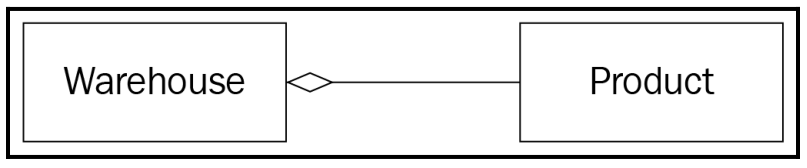
\includegraphics[width=0.4\textwidth]{content/Section-1/Chapter-3/11}
\end{center}

就纯OOP而言,有几种关系,比如关联、聚合、组合、实例化、泛化等。 \par

\noindent\textbf{}\ \par
\textbf{聚合和组合} \ \par
在Warehouse类的示例中遇到了聚合。Warehouse类存储一个Product数组。更一般的术语中,可以称为关联,但为了强调包含,我们使用术语聚合或组合。聚合的情况下,可以在没聚合的情况下实例化包含一个或多个其他类实例的类。这意味着可以创建和使用一个Warehouse对象,而不必创建包含在Warehouse中的Product对象。 \par
聚合的另一个例子是Car和Person。Car可以包含Person对象(作为司机或乘客),因为它们彼此关联,但该包含不是强相关。我们可以创建一个没有Driver的Car对象,如下所示:\par

\begin{lstlisting}[caption={}]
class Person; // forward declaration
class Engine { /* code omitted for brevity */ };
class Car {
	public:
	Car();
	// ...
	private:
	Person* driver_; // aggregation
	std::vector<Person*> passengers_; // aggregation
	Engine engine_; // composition
	// ...
};
\end{lstlisting}

强包容是由组成来表达的。对于Car示例,需要Engine类的对象来创建完整的Car对象。在这个物理表示中,Engine在创建Car时自动创建。 \par
下面是聚合和组合的UML表示: \par

\begin{center}
	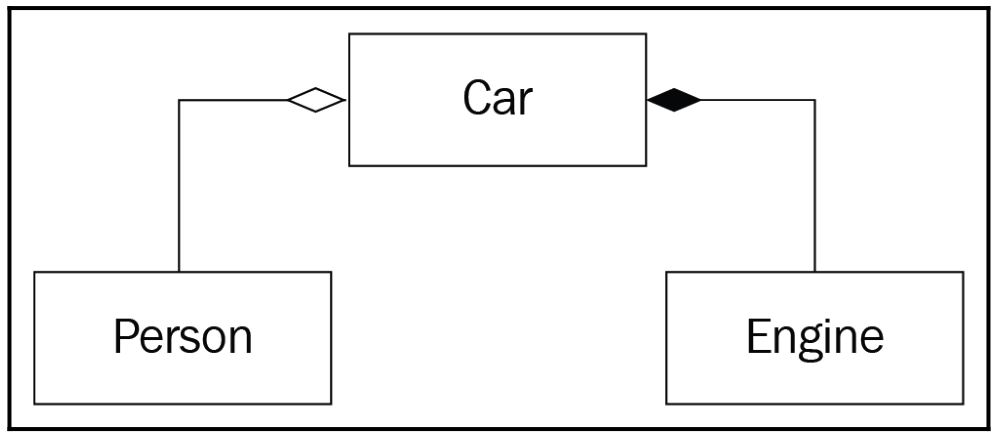
\includegraphics[width=0.4\textwidth]{content/Section-1/Chapter-3/12}
\end{center}

设计类时,我们必须确定它们之间的关系。定义两个类之间的组合的最佳方法是使用has-a关系测试。汽车有引擎,任何时候,你不能决定是否应该用组合的形式来表达这种关系时,就问has-a问题。聚集和组成有些相似,只是描述了这种联系的强度。对于聚合,恰当的问题是可以是,例如:一辆汽车可以有一个司机(Person类型),是弱关联。 \par

\noindent\textbf{}\ \par
\textbf{继承} \ \par
继承是一个编程概念,它允许我们重用类。编程语言提供了不同的继承实现,但一般规则总是成立的:类关系应该回答一个问题。例如,Car就是Vehicle,这让我们可以从Vehicle继承Car: \par

\begin{lstlisting}[caption={}]
class Vehicle {
	public:
	void move();
};
class Car : public Vehicle {
	public:
	Car();
	// ...
};
\end{lstlisting}

Car现在有了从Vehicle派生的move()成员函数。继承本身表示泛化/特化关系,其中父类(Vehicle)是泛化,子类(Car)是特化。 \par

\hspace*{\fill} \\ %插入空行

\includegraphics[width=0.05\textwidth]{images/tip}
父类可以称为基类或超类,而子类可以分别被为派生类或子类(subclass)。 \par
\noindent\textbf{}\ \par

只有在绝对必要时才应该考虑使用继承。正如我们前面提到的,类应该满足is-a关系。考虑Square和Rectangle类,下面的代码以最简单的形式声明了Rectangle类: \par

\begin{lstlisting}[caption={}]
class Rectangle {
public:
	// argument checks omitted for brevity
	void set_width(int w) { width_ = w; }
	void set_height(int h) { height_ = h; }
	int area() const { return width_ * height_; }
private:
	int width_;
	int height_;
};
\end{lstlisting}

正方形是一个矩形,所以我们可以很容易地从矩形继承它: \par

\begin{lstlisting}[caption={}]
class Square : public Rectangle {
public:
	void set_side(int side) {
		set_width(side);
		set_height(side);
	}
	int area() {
		area_ = Rectangle::area();
		return area_;
	}
private:
	int area_;
};
\end{lstlisting}

方形扩展了矩形,添加了一个新的数据成员area\underline{ },并用自己的实现覆盖了area()成员函数。实践中,area\underline{ }和计算值的方法是冗余的,我们这样做是为了演示一个糟糕的类设计,并在一定程度上让Square扩展它的父类。很快,我们将得出这样的结论:在本例中,继承是一个糟糕的选择。Square是一个矩形,所以它应该在任何使用矩形的地方作为矩形使用,如下所示:\par

\begin{lstlisting}[caption={}]
void make_big_rectangle(Rectangle& ref) {
	ref->set_width(870);
	ref->set_height(940);
}

int main() {
	Rectangle rect;
	make_big_rectangle(rect);
	Square sq;
	// Square is a Rectangle
	make_big_rectangle(sq);
}
\end{lstlisting}

make\underline{ }big\underline{ }rectangle()函数接受对矩形的引用,方形继承了它,所以完全可以将一个方形对象发传递给make\underline{ }big\underline{ }rectangle()函数。正方形是一个长方形,成功地用类型的子类型替换的例子称为Liskov替换原则。让我们来看看为什么这个替换在实践中是有效的,然后再决定我们是否有设计错误,从矩形继承了方形。 \par

\noindent\textbf{}\ \par
\textbf{从编译器的角度来看继承} \ \par
我们可以用以下方式来描绘前面声明的Rectangle类: \par

\begin{center}
	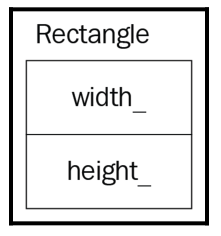
\includegraphics[width=0.2\textwidth]{content/Section-1/Chapter-3/13}
\end{center}

当在main()函数中声明rect时,函数的局部对象所需的空间在堆栈中分配。调用make\underline{ }big\underline{ }rectangle()函数时遵循相同的逻辑。这里没有局部参数,相反,它有一个\texttt{Rectangle\& type}参数,其行为方式与指针类似:获取存储内存地址所需的内存空间(在32位和64位系统中分别为4或8个字节)。rect通过引用传递给make\underline{ }big\underline{ }rectangle(),这意味着ref参数引用main()中的局部对象: \par

\begin{center}
	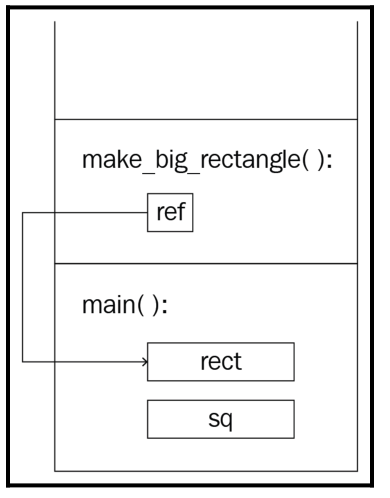
\includegraphics[width=0.4\textwidth]{content/Section-1/Chapter-3/14}
\end{center}

下面是Square类的一个示例: \par

\begin{center}
	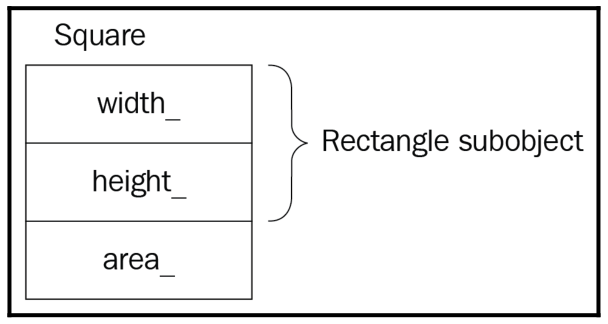
\includegraphics[width=0.4\textwidth]{content/Section-1/Chapter-3/15}
\end{center}

如上图所示,Square对象包含Rectangle的子对象,部分地代表了一个矩形。在这个特定的示例中,Square类没有使用新的数据成员扩展Rectangle。 \par
Square对象传递给make\underline{ }big\underline{ }rectangle(),后者接受\texttt{Rectangle\& type}的参数。我们知道访问基础对象时需要指针(引用)的类型,类型定义了应该从指针所指向的起始地址读取多少字节。这种情况下,ref存储main()中声明的本地rect对象的起始地址的副本。当make\underline{ }big\underline{ }rectangle()通过ref访问成员函数时,实际上调用以Rectangle引用作为第一个形参的全局函数。这个函数转译成如下代码(简单起见,修改了一下): \par

\begin{lstlisting}[caption={}]
void make_big_rectangle(Rectangle * const ref) {
	Rectangle_set_width(*ref, 870);
	Rectangle_set_height(*ref, 940);
}
\end{lstlisting}

解引用ref意味着从ref所指向的内存位置开始读取\texttt{sizeof(Rectangle)}字节。当传递一个Square对象给make\underline{ }big\underline{ }rectangle()时,将sq(Square对象)的起始地址赋值给ref,因为Square对象实际上包含一个Rectangle子对象。当make\underline{ }big\underline{ }rectangle()函数解引用ref时,只能访问对象的\texttt{sizeof(Rectangle)}字节,而看不到实际Square对象的额外字节。下面的图表说明了子对象引用指向的部分: \par

\begin{center}
	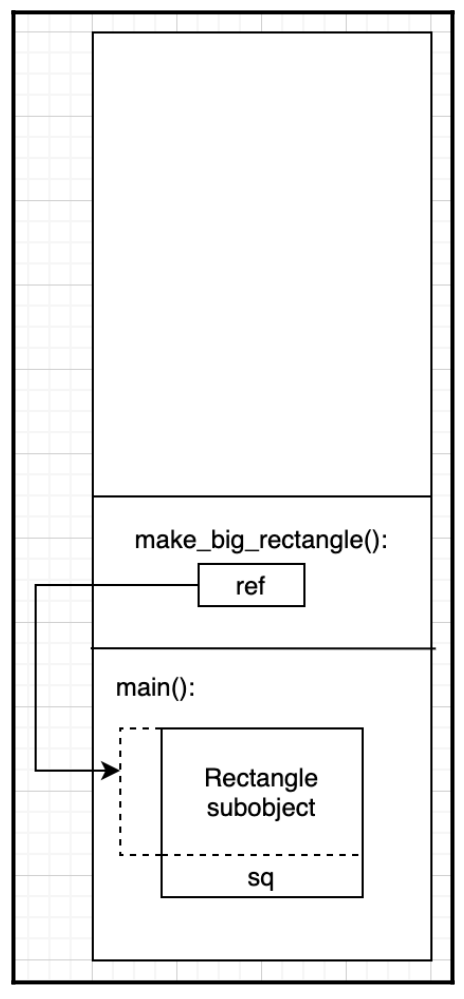
\includegraphics[width=0.4\textwidth]{content/Section-1/Chapter-3/16}
\end{center}

从Rectangle中继承Square等同于声明两个结构体,其中一个(子结构体)包含另一个(父结构体): \par

\begin{lstlisting}[caption={}]
struct Rectangle {
	int width_;
	int height_;
};
void Rectangle_set_width(Rectangle& this, int w) {
	this.width_ = w;
}
void Rectangle_set_height(Rectangle& this, int h) {
	this.height_ = h;
}
int Rectangle_area(const Rectangle& this) {
	return this.width_ * this.height_;
}
struct Square {
	Rectangle _parent_subobject_;
	int area_;
};
void Square_set_side(Square& this, int side) {
	// Rectangle_set_width(static_cast<Rectangle&>(this), side);
	Rectangle_set_width(this._parent_subobject_, side);
	// Rectangle_set_height(static_cast<Rectangle&>(this), side);
	Rectangle_set_height(this._parent_subobject_, side);
}
int Square_area(Square& this) {
	// this.area_ = Rectangle_area(static_cast<Rectangle&>(this));
	this.area_ = Rectangle_area(this._parent_subobject_);
	return this.area_;
}
\end{lstlisting}

前面的代码演示了编译器支持继承的方式。看看Square\underline{ }set\underline{ }side和Square\underline{ }area函数的注释代码行,表达了编译器如何处理OOP代码的全部思想。 \par

\noindent\textbf{}\ \par
\textbf{组合和继承} \ \par
C++语言为提供了方便且对OOP友好的语法,这样就可以表达继承关系,但是编译器处理它的方式类似于组合而不是继承。实际上,在适用的情况下,使用组合而不是继承会更好。Square类及其与矩形的关系是一个糟糕的设计。原因是子类型替换原则,我们以错误的方式使用Square:将其传递给一个函数,该函数将其修改为Rectangle而不是Square。这告诉我们,is-a关系是不正确的,因为Square毕竟不是Rectangle。它是对Rectangle的泛化,而不是Rectangle。\par
使用Square的用户最好不了解它可以作为Rectangle使用,否则将向Square实例发送无效或不受支持的消息。无效消息的例子是调用set\underline{ }width或set\underline{ }height函数。Square实际上不应该支持两个不同的成员函数来修改它的边长,但它不能隐藏这一点,因为它继承自Rectangle: \par

\begin{lstlisting}[caption={}]
class Square : public Rectangle {
	// code omitted for brevity
};
\end{lstlisting}

如果我们把修饰语从public改为private会怎样?C++既支持公有继承类型,也支持私有继承类型,还支持受保护的继承。当私有继承一个类时,子类打算使用父类并访问其公共接口。但是,客户端代码并不知道它在处理一个派生类。此外,从父类继承的公共接口对于子类的用户来说变成了私有的。看起来像是将继承转换成组合:\par

\begin{lstlisting}[caption={}]
class Square : private Rectangle {
public:
	void set_side(int side) {
		// Rectangle's public interface is accessible to the Square
		set_width(side);
		set_height(side);
	}
	int area() {
		area_ = Rectangle::area();
		return area_;
	}
private:
	int area_;
};
\end{lstlisting}

客户端代码不能访问从Rectangle继承的成员: \par

\begin{lstlisting}[caption={}]
Square sq;
sq.set_width(14); // compile error, the Square has no such public member
make_big_rectangle(sq); // compile error, can't cast Square to Rectangle
\end{lstlisting}

同样可以通过在Square的私有部分声明一个Rectangle成员来实现: \par

\begin{lstlisting}[caption={}]
class Square {
public:
	void set_side(int side) {
		rectangle_.set_width(side);
		rectangle_.set_height(side);
	}
	int area() {
		area_ = rectangle_.area();
		return area_;
	}
private:
	Rectangle rectangle_;
	int area_;
};
\end{lstlisting}

为了使用继承,应该仔细分析使用场景,并回答is-a问题。每当要在组合和继承之间做出选择时,请选择组合。 \par
当私有继承时,可以省略修饰符。类的默认访问修饰符是private,所以\texttt{class Square: private Rectangle \{\};}与\texttt{class Square: Rectangle \{\};}相反,struct的默认修饰符是public。\par

\noindent\textbf{}\ \par
\textbf{保护继承} \ \par
最后是带protected修饰符的继承,指定在类主体中使用的类成员的访问级别。受保护的成员对类用户是私有的,但对派生类是公有的。如果修饰符用于指定继承类型,则它的行为类似于派生类用户的私有继承。私有继承向所有派生类用户隐藏基类的公共接口,而受保护继承使派生类的后代可以访问基类。 \par
很难想象需要受保护的继承的场景,但您应该将其视为一种工具,它可能在意想不到的明显设计中有用。让我们假设我们需要设计一个堆栈数据结构适配器。堆栈通常基于向量(一维数组)、链表或队列来实现。 \par

\hspace*{\fill} \\ %插入空行

\includegraphics[width=0.05\textwidth]{images/tip}
堆栈符合后进先出规则,即插入到堆栈中的最后一个元素将首先访问。类似地,插入到堆栈中的第一个元素将最后访问。我们将在第6章更详细地讨论数据结构和数据结构适配器。 \par
\noindent\textbf{}\ \par

栈本身并不代表数据结构,它位于数据结构之上,并通过限制、修改或扩展其功能来调整其使用。下面是Vector类的一个简单声明,表示一维整数数组:\par

\begin{lstlisting}[caption={}]
class Vector {
public:
	Vector();
	Vector(const Vector&);
	Vector(Vector&&);
	Vector& operator=(const Vector&);
	Vector& operator=(Vector&&);
	~Vector();
public:
	void push_back(int value);
	void insert(int index, int value);
	void remove(int index);
	int operator[](int index);
	int size() const;
	int capacity() const;
private:
	int size_;
	int capacity_;
	int* array_;
};
\end{lstlisting}

前面的Vector不是支持随机访问迭代器的STL兼容容器,包含动态递增数组的最小值。它可以通过以下方式声明和使用:\par

\begin{lstlisting}[caption={}]
Vector v;
v.push_back(4);
v.push_back(5);
v[1] = 2;
\end{lstlisting}

Vector类提供了操作符[],允许随机访问任何项,而堆栈禁止随机访问。栈提供了push和pop操作,因此可以分别向其底层数据结构中插入一个值并获取该值:\par

\begin{lstlisting}[caption={}]
class Stack : private Vector {
	public:
	// constructors, assignment operators and the destructor are omitted for	brevity
	void push(int value) {
		push_back(value);
	}
	int pop() {
		int value{this[size() - 1]};
		remove(size() - 1);
		return value;
	}
};
\end{lstlisting}

栈的使用方式如下: \par

\begin{lstlisting}[caption={}]
Stack s;
s.push(5);
s.push(6);
s.push(3);
std::cout << s.pop(); // outputs 3
std::cout << s.pop(); // outputs 6
s[2] = 42; // compile error, the Stack has no publicly available operator[]
defined
\end{lstlisting}

堆栈自适应Vector,并提供两个成员函数,以便可以访问。私有继承允许使用Vector的全部功能,并向堆栈用户隐藏继承信息。如果想要继承堆栈来创建它的高级版本,该怎么办?假设AdvancedStack类提供了min()函数,该函数在常量时间内返回堆栈中包含的最小值。\par
私有继承禁止AdvancedStack,使用Vector的公共接口,因此需要一种方法允许Stack子类使用基类,但对类用户隐藏基类的存在。保护继承实现了这一目标,如下面的代码所示: \par

\begin{lstlisting}[caption={}]
class Stack : protected Vector {
	// code omitted for brevity
};
class AdvancedStack : public Stack {
	// can use the Vector
};
\end{lstlisting}

通过从Vector继承堆栈,允许堆栈的子类使用Vector公共接口。但是堆栈和AdvancedStack的用户都不能以向量的形式访问。 \par

\noindent\textbf{}\ \par
\textbf{多态性} \ \par
多态是面向对象编程中的另一个关键概念,允许子类拥有自己的基类派生函数的实现。假设我们有一个Musician类,它有play()成员函数: \par

\begin{lstlisting}[caption={}]
class Musician {
	public:
	void play() { std::cout << "Play an instrument"; }
};
\end{lstlisting}

现在,声明一个Guitarist类,它有play\underline{ }guitar()函数: \par

\begin{lstlisting}[caption={}]
class Guitarist {
	public:
	void play_guitar() { std::cout << "Play a guitar"; }
};
\end{lstlisting}

这是使用继承的明显例子,因为Guitarist是一个Musician。Guitarist自然不会通过添加新函数(如play\underline{ }guitar())来扩展Musician。相反,应该提供自己从Musician派生的play()函数的实现。为此,我们使用虚函数: \par

\begin{lstlisting}[caption={}]
class Musician {
public:
	virtual void play() { std::cout << "Play an instrument"; }
};
class Guitarist : public Musician {
public:
	void play() override { std::cout << "Play a guitar"; }
};
\end{lstlisting}

现在,Guitarist类提供了自己的play()函数实现,客户端代码可以通过使用基类的指针访问它: \par

\begin{lstlisting}[caption={}]
Musician armstrong;
Guitarist steve;
Musician* m = &armstrong;
m->play();
m = &steve;
m->play();
\end{lstlisting}

前面的例子展示了多态性的实际应用。虽然虚函数的使用很自然,但除非我们正确地使用它,否则它实际上没有多大意义。首先,Musician的play()函数不应该有任何实现。原因很简单:音乐家应该能够演奏一种具体的乐器,因为他们不能同时演奏一种以上的乐器。为了避免实现,我们将函数设置为纯虚函数,为其赋值0: \par

\begin{lstlisting}[caption={}]
class Musician {
	public:
	virtual void play() = 0;
};
\end{lstlisting}

当客户端代码试图声明音乐家的实例时,这会导致编译错误,因为不能够创建一个具有未定义函数的对象。Musician的作用只有一个:只能继承。存在的要继承的类称为抽象类。实际上,Musician称为接口,而不是抽象类。抽象类是一种半接口半类的存在,可以拥有两种类型的函数:有实现的函数和没有实现的函数。\par
回到我们的例子,让我们添加Pianist类,它也实现了Musician接口:\par

\begin{lstlisting}[caption={}]
class Pianist : public Musician {
	public:
	void play() override { std::cout << "Play a piano"; }
};
\end{lstlisting}

为了表达多态性的全部,假设在某个地方声明了一个函数,它返回一个Musician的集合,Guitarist或Pianist: \par

\begin{lstlisting}[caption={}]
std::vector<Musician*> get_musicians();
\end{lstlisting}

从客户端代码的角度来看,很难分析get\underline{ }musicians()函数的返回值并找出对象的实际子类型。可能是吉他手或钢琴家,甚至是一个纯粹的音乐家。关键是客户端不应该真正关心对象的实际类型,因为它知道集合中包含了乐手,而且乐手对象具有play()函数。因此,要让它们发挥作用,客户机只需遍历这个集合,并让每个乐师演奏它的乐器(每个对象调用它的实现):\par

\begin{lstlisting}[caption={}]
auto all_musicians = get_musicians();
for (const auto& m: all_musicians) {
	m->play();
}
\end{lstlisting}

前面的代码表达了多态性的全部功能。现在,让我们了解该如何在语言在底层支持多态。 \par

\noindent\textbf{}\ \par
\textbf{虚函数} \ \par
尽管多态性并不局限于虚函数,但我们将它们放在一起讨论。再次强调,更好地理解概念或技术的最好方法是自己实现它。无论是在类中声明虚成员函数,还是在基类中声明虚函数,编译器都会给该类增加一个额外的指针。指针指向一个表,这个表通常称为虚函数表,或者简单地称为虚表。我们也将该指针称为虚表指针。 \par
我们假设我们正在为银行客户账户管理实现一类子系统。假设银行要求我们根据帐户类型实现兑现。例如,储蓄账户允许每年提现一次,而支票账户允许客户随时提现。在不了解任何关于Account类(不必要的)细节的情况下,让我们声明一个可以帮助理解虚拟成员函数的最小构造。让我们看看Account类的定义: \par

\begin{lstlisting}[caption={}]
class Account
{
public:
	virtual void cash_out() {// the default implementation for cashing out
	}
	virtual ~Account() {}
private:
	double balance_;
};
\end{lstlisting}

编译器将Account类转换为一个具有指向虚函数表指针的结构。下面的代码代表伪代码,解释了当我们在类中声明虚函数时会发生什么。和往常一样,请注意提供的是通用的解释,而不是特定于编译器的实现(名称重置整也是通用形式,例如:将cash\underline{ }out更名为Account\underline{ }cash\underline{ }out): \par

\begin{lstlisting}[caption={}]
struct Account
{
	VTable* __vptr;
	double balance_;
};

void Account_constructor(Account* this) {
	this->__vptr = &Account_VTable;
}

void Account_cash_out(Account* this) {
	// the default implementation for cashing out
}

void Account_destructor(Account* this) {}
\end{lstlisting}

仔细看看前面的伪代码。Account结构体的第一个成员是\underline{~~}vptr。由于前面声明的Account类有两个虚函数,所以可以将虚表想象为一个数组,其中有两个指向虚成员函数的指针。详见以下表示:\par

\begin{lstlisting}[caption={}]
VTable Account_VTable[] = {
	&Account_cash_out,
	&Account_destructor
};
\end{lstlisting}

根据之前的假设,看看在对象上调用虚函数时编译器会生成什么代码: \par

\begin{lstlisting}[caption={}]
// consider the get_account() function as already implemented and returning
an Account*
Account* ptr = get_account();
ptr->cash_out();
\end{lstlisting}

下面是我们可以想象的编译器生成的代码和前面的代码是一样的: \par

\begin{lstlisting}[caption={}]
Account* ptr = get_account();
ptr->__vptr[0]();
\end{lstlisting}

虚函数在层次结构中使用时显示了它们的威力。SavingsAccount从Account类继承如下: \par

\begin{lstlisting}[caption={}]
class SavingsAccount : public Account
{
public:
	void cash_out() override {
		// an implementation specific to SavingsAccount
	}
	virtual ~SavingsAccount() {}
};
\end{lstlisting}

当通过指针(或引用)调用cash\underline{ }out()时,虚函数将基于指针所指向的目标对象调用。例如,假设get\underline{ }savings\underline{ }account()返回一个SavingsAccount为Account*。下面的代码将调用cash\underline{ }out()的SavingsAccount实现: \par

\begin{lstlisting}[caption={}]
Account* p = get_savings_account();
p->cash_out(); // calls SavingsAccount version of the cash_out
\end{lstlisting}

下面是编译器为SavingsClass生成的内容: \par

\begin{lstlisting}[caption={}]
struct SavingsAccount
{
	Account _parent_subobject_;
	VTable* __vptr;
};
VTable* SavingsAccount_VTable[] = {
	&SavingsAccount_cash_out,
	&SavingsAccount_destructor,
};
void SavingsAccount_constructor(SavingsAccount* this) {
	this->__vptr = &SavingsAccount_VTable;
}
void SavingsAccount_cash_out(SavingsAccount* this) {
	// an implementation specific to SavingsAccount
}
void SavingsAccount_destructor(SavingsAccount* this) {}
\end{lstlisting}

我们有两个不同的虚函数表。当创建Account类型的对象时,它的\underline{~~}vptr指向Account\underline{ }VTable,而SavingsAccount类型的对象的\underline{ ~~}vptr指向SavingsAccount\underline{ }VTable。让我们来看看下面的代码: \par

\begin{lstlisting}[caption={}]
p->cash_out();
\end{lstlisting}

前面的代码转译成这样: \par

\begin{lstlisting}[caption={}]
p->__vptr[0]();
\end{lstlisting}

现在,很明显\underline{~~}vptr[0]解析为正确的函数,因为它是通过p指针读取的。\par
如果SavingsAccount没有覆盖cash\underline{ }out()函数怎么办?在这种情况下,编译器只是将基类实现的地址与SavingsAccount\underline{ }VTable放在同一个槽中,如下所示:\par

\begin{lstlisting}[caption={}]
VTable* SavingsAccount_VTable[] = {
	// the slot contains the base class version
	// if the derived class doesn't have an implementation
	&Account_cash_out,
	&SavingsAccount_destructor
};
\end{lstlisting}

编译器以不同的方式实现虚拟函数的表示和管理。有些实现甚至使用不同的模型,而不是我们前面介绍的模型。我们引入了一种流行的方法,为了简单起见,我们用通用的方式来表示它。现在,我们将看看在包含动态多态性的代码背后发生了什么。\par

\noindent\textbf{}\ \par
\textbf{设计模式} \ \par
设计模式是程序员最具表现力的工具之一,允许我们以一种优雅且经过良好测试的方式解决设计问题。当努力提供类及其关系的最佳设计时,著名的设计模式可能会帮助您。 \par
设计模式最简单的例子是单例。它为我们提供了一种声明和使用类的一个实例的方法,例如:假设电子商务平台只有一个仓库。为了访问Warehouse类,项目可能要求我们在许多源文件中包含并使用它。为了保持同步,我们应该将仓库设置为单例: \par

\begin{lstlisting}[caption={}]
class Warehouse {
public:
	static create_instance() {
		if (instance_ == nullptr) {
			instance_ = new Warehouse();
		}
		return instance_;
	}
	static remove_instance() {
		delete instance_;
		instance_ = nullptr;
	}
private:
	Warehouse() = default;
private:
	static Warehouse* instance_ = nullptr;
};
\end{lstlisting}

我们声明了一个静态Warehouse对象,和两个用于创建和销毁相应实例的静态函数。每当用户试图以旧的方式声明Warehouse对象时,private构造函数都会阻止编译。为了能够使用Warehouse,客户端代码必须调用create\underline{ }instance()函数: \par

\begin{lstlisting}[caption={}]
Warehouse* w = Warehouse::create_instance();
Product book;
w->add_product(book);
Warehouse::remove_instance();
\end{lstlisting}

Warehouse的单例实现并不完整,只是一个引入设计模式的示例。我们将在本书中介绍更多的设计模式。\par

\noindent\textbf{}\ \par
\textbf{总结} \ \par
本章中,我们讨论了面向对象编程的基本概念。讨论了类的底层细节和C++对象模型的编译器实现。知道如何在没有实际类的情况下,设计和实现类对正确使用类有很大帮助。\par
我们还讨论了对继承的需求,并尝试在可能适用的情况下使用组合而不是继承。C++支持三种类型的继承:公有、私有和保护。所有这些类型在特定的类设计中都有它们的应用。最后,我们通过一个例子来理解多态性的使用和强大功能,这个例子极大地增加了客户机代码的便利性。 \par
下一章中,我们将学习更多关于模板和模板元编程的知识,我们将以此为基础深入研究C++20的一个新特性,这个特性叫做概念。 \par

\noindent\textbf{}\ \par
\textbf{问题} \ \par
\begin{enumerate}
	\item 对象的三个属性是什么?
	\item 移动对象比复制对象有什么优势?
	\item C++中,结构和类有什么区别?
	\item 聚合关系和合成关系有什么区别?
	\item 私有继承和受保护的继承有什么区别?
	\item 如果在类中定义虚函数,类的大小会受到什么影响?
	\item 使用单例设计模式的意义是什么?
\end{enumerate}

\noindent\textbf{}\ \par
\textbf{扩展阅读} \ \par
更多信息,请参阅: \par

\begin{itemize}
	\item Grady Booch,面向对象的分析和设计》( https:/​/www.​amazon.​com/Object-​Oriented-​Analysis-​Design-​Applications-​3rd/​dp/​020189551X/​ )
	\item Stanley Lippman,《C++对象的内部模型》 ( https:/​/​www.​amazon.​com/​Inside-	Object-​Model-​Stanley-​Lippman/​dp/​0201834545/​ )
\end{itemize}

\newpage



















